\section{Appendix}\label{appendix}
    \subsection{Standardization of Lasso}\label{standardization_of_lasso}
         In this section, we attempt to show that a standardization of regressors is required for an effective variable selection in Lasso. We use the same setting as shown in Section \ref{lasso}. $(Z_1, Y_1), \ldots, (Z_n,Y_n)$ is iid data with $Z_i \in \mathbb{R}^p$ and $Y_i \in \mathbb{R}$, following a linear model.
        \begin{align*}\label{linear_model}
            Y=\sum\limits_{j=1}^p Z_j\beta_j+\epsilon
        \end{align*}

        where $\beta_j$ are unknown coefficients. $Y=(Y_1, Y_2, \ldots, Y_n)^T$, $Z_j=(Z_{1j}, Z_{2j}, \ldots, Z_{nj})^{T}$ and $E[\epsilon|Z_1, Z_2, \ldots, Z_n]=0$. To save notation in the proof, we further assume that $Z_i$ does not contain a constant. Also, we have an orthonormality design, i.e., regressors are mutually orthonormal. To put it formally,
        \begin{align*}
            \frac{1}{n}Z^TZ=
            \begin{pmatrix}
                1 & 0 & \ldots & 0 \\
                0 & 1 & \ldots & 0 \\
                \vdots & \vdots & \ddots & \vdots \\
                0 & 0 & \ldots & 1 \\
            \end{pmatrix}
        \end{align*}
        where $Z=(Z_1,Z_2, \ldots, Z_j)$. Variances of all regressors $Z_j$ are normalized to 1. In this orthonormal design, it can be easily shown\footnote{Please refer to Section 2.4.1, \cite{Hastie_Tibshirani_Wainwright_2015} for details.} that a lasso estimate $\hat{\beta}_{\lambda, j}$ is
        \begin{align*}
            \hat{\beta}_{\lambda, j}=
            \begin{cases}
                \hat{\beta}_{OLS, j} + \lambda & \text{, if $\hat{\beta}_{OLS, j} < -\lambda$}\\
                0 & \text{, if $|\hat{\beta}_{OLS, j}| \le \lambda$}\\
                \hat{\beta}_{OLS, j} - \lambda & \text{, if $\hat{\beta}_{OLS, j} > \lambda$}\\
            \end{cases}
        \end{align*}
        where $\hat{\beta}_{OLS, j}=\frac{1}{n}\sum_{i=1}^n Z_{ij}Y_i$ is the coefficients estimated by OLS in this orthonormal design. It is seen that Lasso only selects regressor $Z_j$ if $|\hat{\beta}_{OLS, j}|=|\frac{1}{n}\sum_{i=1}^n Z_{ij}Y_i|>\lambda$. It means that the selection rule depends on the scale of coefficients. For example, if $Z_{1}$ is centered at 10000, while $Z_{2}$ is centered at 0, Lasso would unfairly prefer to selecting $Z_{1}$ since $|\frac{1}{n}\sum_{i=1}^n Z_{i1}Y_i|>\lambda$ even for a large $\lambda$. To remove such an unfair influence, it is required to standardize regressors beforehand.
        \begin{align*}
            \tilde{Z}_{ij}=\frac{Z_{ij}-\bar{Z}_j}{\hat{\sigma}_j}
        \end{align*}
        where $\hat{\sigma}_j$ is the standard deviation of $Z_j$. By using standardized $\tilde{Z}_{ij}$, the selection rule is not affected by the magnitude of variables, thus achieving an effective variable selection.
        


    \subsection{Derivation of $\kappa_M$ in Assumption \ref{dae_assumption_3}}\label{derivation_kappa}
        Let $g_k(X)=\prod_{l=1}^d p_{k_l}(x_l)$ denote basis functions with $1 \le k \le M$, and $g^M(X)=(g_1(X), \ldots, g_M(X))^T$ is the vector of all basis functions. Then, $\Psi_M=E[g^M(X)g^M(X)^{T}]$ in our setting. Let $v \in \mathbb{R}^M$, then
        \begin{align*}
            v^{T}\Psi_M v =& v^{T} E[g^M(X)g^M(X)^{T}]v\\
            =& E[(v^{T}g^M(X))^2]\\
            \ge & \frac{1}{C} \int_{\mathcal{X}}(v^{T}g^M(x))^2 dx\\
            = & \frac{1}{C} \int_{\mathcal{X}} \sum_{k=1}^{M}\sum_{j=1}^{M}v_kv_jg_k(x)g_j(x) dx\\
            = & \frac{1}{C}\sum_{k=1}^{M}v_k^2\\
            = & \frac{1}{C}v^{T}v
        \end{align*}

        To move from the second to the third line, we use the assumption that $||g_k(X)||=||\prod_{l=1}^d p_{k_l}(x_l)|| \ge c_0 = \frac{1}{C}$. To move from the fourth to fifth line, we use the orthonormality property of our basis functions. Moreover, 
        \begin{align*}
            v^{T}\mathrm{diag}(\Psi_M)v \le & C \int_{\mathcal{X}}\sum_{k=1}^M v_k^2 g_k(x)^2 dx\\
            =& C \sum_{k=1}^M v_k^2 \int_{\mathcal{X}} g_k(x)^2 dx\\
            =& Cv^{T}v
        \end{align*}

        In the first line, we use the assumption that $||g_k(X)||=||\prod_{l=1}^d p_{k_l}(x_l)|| \le C$. It follows that for any non-zero real vector $v$, we have
            \begin{align*}
                v^{T}\left(\Psi-\frac{1}{C^2}\mathrm{diag}(\Psi_M)\right)v=&v^{T}\Psi_Mv-\frac{1}{C^2}v^{T}\mathrm{diag}(\Psi_M)v\\
                \ge & \frac{1}{C}v^{T}v-\frac{1}{C}v^{T}v\\
                =&0
            \end{align*}
                        
        Therefore, there exists a constant $\kappa_M=\frac{1}{C^2}>0$ such that $\Psi_M-\kappa_M\mathrm{diag}(\Psi_M)$ is positive semi-definite. Assumption \ref{assumption_3} is thus guaranteed. It is noted that orthonormality of basis functions simplifies the expression of $\kappa_M$, but even if basis functions are not orthonormal, there can exist such a $\kappa_M>0$ that makes $\Psi_M-\kappa_M\mathrm{diag}(\Psi_M)$ positive semi-definite, though probably with a more complicated derivation process and expression.

    \subsection{Proof of Corollary \ref{smoothness_corollary}}\label{proof_of_corollary}
        \subsubsection{Normalized Legendre Polynomials}\label{normalized_legendre}

        \textbf{Step 1: Deriving $L$ and $L_0$ in Assumption \ref{dae_assumption_2}}\\
        By definition, Legendre polynomials are orthogonal with respect to a uniform density on $[-1,1]$ (\cite{Hansen_2022}). Suppose $p_k(X)$ ($k=0,1,2,\ldots$) are Legendre polynomials defined on interval $[-1,1]$. By fixing $p_k(1)=1$, we have\footnote{\url{https://en.wikipedia.org/wiki/Legendre_polynomials}}:
        \begin{align*}
            \int_{-1}^1 p_j(x)p_k(x)\diff x=\frac{2}{2k+1} \delta_{jk}
        \end{align*}
        where $\delta_{jk}$ denotes Kronecker delta\footnote{Kronecker delta is a function of two variables, which are usually non-negative integers. The function is 1 if the two variables equal, and is 0 otherwise. For example, $\delta_{12}=0$, because $1 \not= 2$; while $\delta_{11}=1$, because $1=1$.}, which equals to 1 if $j=k$, and equals to 0 otherwise. That means, the squared $L_2$ norm of $p_k(X)$ on $[-1,1]$ is:
        \begin{align*}
            ||p_k(X)||^2=\int_{-1}^1 p_k(x)^2 \diff x = \frac{2}{2k+1}
        \end{align*}
        where $||\cdot||$ denotes $L_2$ norm. Then, if we further normalize the Legendre polynomials $p_k(X)$, we have $\tilde{p}_k(X)=\sqrt{\frac{2k+1}{2}}p_k(X)$ such that:
        \begin{align*}
            ||\tilde{p}_k(X)||^2=\int_{-1}^1 \tilde{p}_k(X)^2 \diff x =\int_{-1}^1 \left(\sqrt{\frac{2k+1}{2}}p_k(x)\right)^2 \diff x =\frac{2k+1}{2}||p_k(X)||^2=1
        \end{align*}
        Therefore, $\tilde{p}_k(X)$ ($k=0,1,2,\ldots$) are normalized Legendre polynomials that are discussed in Corollary \ref{smoothness_corollary}. They are orthonormal. In Figure \ref{legendre_poly_plot}, it is seen that Legendre polynomials $p_k(X)$ are bounded above by 1, so for normalized Legendre polynomials, we have:
        \begin{align*}
            ||\tilde{p}_k(X)||_{\infty}=\left|\left|\sqrt{\frac{2k+1}{2}}p_k(X)\right|\right|_{\infty} \le \sqrt{\frac{2k+1}{2}}
        \end{align*}
         In other words, $||\tilde{p}_k||_{\infty} \lesssim \sqrt{k}$. As a consequence, the $L_{\infty}$ norm of basis functions in our multivariate sieve space is $||\prod_{l=1}^d \tilde{p}_{k_l}||_{\infty} \lesssim \sqrt{\prod_{l=1}^dk_l}$. Because $\sum_{l=1}^dk_l \lesssim n^{\frac{1}{2\underline{s}+1}}$ with reference to (\ref{set_of_basis_function}), we can maximize the product $\prod_{l=1}^dk_l$ by having $k_l=\frac{1}{d}n^{\frac{1}{2\underline{s}+1}}$. Then,
         \begin{align*}
             \left|\left|\prod_{l=1}^d \tilde{p}_{k_l}\right|\right|_{\infty} \lesssim n^{\frac{d}{4\underline{s}+2}}
         \end{align*}
         As a result, according to Assumption \ref{dae_assumption_2}, we have $L=n^{\frac{d}{4\underline{s}+2}}$ and $L_0=L^2=n^{\frac{d}{2\underline{s}+1}}$.\\

        \textbf{Step 2: Discussing the first part of inequality about $\pi_{n,M}(\beta)$ in (\ref{pi_n_M})}
        
        To make $\pi_{n,M}(\beta)$ asymptotically zero, it is sufficient to make its upper bound to be asymptotically zero. There are two parts in its upper bound, then it is sufficient to have both parts going to zero in the limit. Ignoring constants, the first part of upper bound of $\pi_{n,M}(\beta)$ is
        \begin{align*}
            &M^2\exp\left( -\min\left\{ nr_{n,M}^2, \frac{nr_{n,M}}{L}, \frac{n}{L^2}, \frac{n}{L_0M^2(\beta)},\frac{n}{L^2M(\beta)} \right\} \right)\\
            =& M^2 \exp\left( -\min\left\{ A^2\log M, A \sqrt{\log M} n^{\frac{1}{2}-\frac{d}{4\underline{s}+2}}, n^{1-\frac{d}{2\underline{s}+1}},n^{1-\frac{d}{2\underline{s}+1}}M^{-2}(\beta), n^{1-\frac{d}{2\underline{s}+1}}M^{-1}(\beta)\right\} \right)\\
            =& M^2 \exp\left( -\min\left\{ A^2\log M, A \sqrt{\log M} n^{\frac{1}{2}-\frac{d}{4\underline{s}+2}}, n^{1-\frac{d}{2\underline{s}+1}},n^{1-\frac{d}{2\underline{s}+1}-\frac{2d}{2s+d}}, n^{1-\frac{d}{2\underline{s}+1}-\frac{d}{2s+d}}\right\} \right)
        \end{align*}
        To move from the first to second line, we use $L=n^{\frac{d}{4\underline{s}+2}}$ and $L_0=n^{\frac{d}{2\underline{s}+1}}$ for normalized Legendre polynomials. To move from the second to third line, we use $M(\beta)=n^{\frac{d}{2s+d}}$ because it is the largest among all three types of underlying models. A sufficient condition for this upper bound to be asymptotically zero is that all terms within the brace should go to infinity, otherwise the upper bound is not asymptotically zero. The terms $A^2\log M$ is naturally non-zero. Then the sufficient condition is reduced to
        \[
        \left\{
            \begin{array}{cc}
                \frac{1}{2}-\frac{d}{4\underline{s}+2} & \ge0 \\
                1-\frac{d}{2\underline{s}+1} & >0 \\
                1-\frac{d}{2\underline{s}+1}-\frac{2d}{2s+d} & > 0\\
                1-\frac{d}{2\underline{s}+1}-\frac{d}{2s+d}& > 0\\
                \underline{s}&\ge0\\
            \end{array}
        \right.
        \]
        If this set of inequalities works for $\underline{s}$, then it should work for all $s$. So, we can replace $s$ with $\underline{s}$. Then, by solving this set of inequalities, we have
        \begin{align*}
            \underline{s} > \frac{2d-1+\sqrt{8d^2+1}}{4}
        \end{align*}
        For example, when $d=2$, we need $\underline{s}>2.187$ to maintain the optimal convergence rate in Theorem \ref{convergence_rates_theorem}. The formula is a little bit complicated, but we can find a simpler sufficient condition.
        \begin{align*}
            \underline{s}\ge\frac{3d-1}{2}
        \end{align*}
        This is a sufficient condition because $\frac{3d-1}{3}>\frac{2d-1+\sqrt{8d^2+1}}{4}$ for all $d \in \{1,2,\ldots\}$. It is worthy of mentioning that the above condition is derived from using $M(\beta)=n^{\frac{d}{2s+d}}$, which is the largest $M(\beta)$ in all three underlying models. \\
                        
        Hence, even if $\underline{s} \le \frac{2d-1+\sqrt{8d^2+1}}{4}$, it can still help to maintain the optimal convergence rate in additive and parametric model. By following a similar argument as above but with $M(\beta)=n^{\frac{1}{2\underline{s}+1}}$, we have a sufficient condition $\underline{s}\ge \frac{d+1}{2}$, which is smaller than the lower bound for maintaining convergence rate in all three models. Likewise, if we only need the optimal convergence rate to hold in parametric model, then we can use $M(\beta)=K^d$ with $K$ being a positive constant. The resulting condition is $\underline{s}> \frac{d-1}{2}$. \\

        \textbf{Step 3: Discussing the second part of inequality about $\pi_{n,M}(\beta)$ in (\ref{pi_n_M})}

        Regarding the second part of upper bound of $\pi_{n,M}(\beta)$, we have
        \begin{align*}
            \exp\left( -\frac{M(\beta)}{L^2(\beta)}nr_{n,M}^2 \right)=\exp\left( -\frac{M(\beta)}{L^2(\beta)}A^2\log M \right)
        \end{align*}
        where $L(\beta)=||f-f_{\beta}||_{\infty}$. With reference to the formula (3.7) in \cite{Belloni_Chernozhukov_Chetverikov_Kato_2015}, we have $L(\beta) \lesssim M(\beta)^{-\frac{s}{d}}$. Then, 
        \begin{align*}
            \frac{M(\beta)}{L^2(\beta)} \gtrsim M(\beta)^{\frac{2s+d}{d}} = n^{\frac{d}{2s+d}\frac{2s+d}{d}}=n
        \end{align*}
        where we use $M(\beta)=n^{\frac{d}{2s+d}}$. Obviously, the second part is asymptotically zero, too. The result also holds when $M(\beta)=n^{\frac{1}{2s+1}}$ or $K^d$. The intuitive explanation is that when $n \rightarrow \infty$, the $L_{\infty}$ norm of approximation error $L(\beta)$ goes to zero, and the number of coefficients $M(\beta)$ goes to infinity, thus making $\frac{M(\beta)}{L^2(\beta)}$ goes to infinity. 
        
        \subsubsection{Orthonormalized B-Splines}\label{orthonormalized_b-splines}

        \textbf{Step 1: Deriving $L$ and $L_0$ in Assumption \ref{dae_assumption_2}}\\
        In Appendix \ref{orthogonal_b_splines}, it is shown that on $[a,b]$, the squared $L_2$ norm of orthogonal B-Splines $||P_k||^2$ are bounded above. From the example in Table \ref{example_values_n_k}, it is further observed that $||P_k||^2$ grows with $k$. Hence, if $P_k$ is normalized, the resulting orthonomalized B-Splines $\tilde{P}_k$ would have an $L_{\infty}$ norm that goes downward with $k$. Then, it is bounded above, supposedly by a constant $C$. As a consequence, the $L_{\infty}$ norm of basis functions in multivariate sieve space is $||\prod_{l=1}^d \tilde{P}_{k_l}||_{\infty} \lesssim C^d$. According to Assumption \ref{dae_assumption_2}, we have $L=C^d$ and $L_0=L^2=C^{2d}$. \\
    
        \textbf{Step 2: Discussing the first part of inequality about $\pi_{n,M}(\beta)$ in (\ref{pi_n_M})}\\
        Again, it is sufficient to argue that both parts of the upper bound of $\pi_{n,M}(\beta)$ goes to zero in the limit. Ignoring constants, the first part is
        \begin{align*}
            &M^2\exp\left( -\min\left\{ nr_{n,M}^2, \frac{nr_{n,M}}{L}, \frac{n}{L^2}, \frac{n}{L_0M^2(\beta)},\frac{n}{L^2M(\beta)} \right\} \right)\\
            =& M^2\exp\left( -\min\left\{ A^2 \log M, A\sqrt{\log M}C^{-d}n, C^{-2d}n, C^{-2d}nM^{-2}(\beta), C^{-2d}nM^{-1}(\beta) \right\} \right)\\
            =& M^2\exp\left( -\min\left\{ A^2 \log M, A\sqrt{\log M}C^{-d}n, C^{-2d}n, C^{-2d}n^{1-\frac{2d}{2s+d}}, C^{-2d}n^{1-\frac{d}{2s+d}} \right\} \right)
        \end{align*}

        To move from the first to second line, we use $L=C^d$ and $L_0=C^{2d}$ for orthonormalized B-splines. To move from the second to third line, we use $M(\beta)=n^{\frac{d}{2s+d}}$ because it is the largest among all three underlying models. Again, a sufficient condition is that all terms should go to infinity. The terms $A^2 \log M$, $A\sqrt{\log M}C^{-d}n$ and $C^{-2d}n$ are nonzero, so the condition is reduced to 
        \[
            \left\{
            \begin{array}{cc}
                1-\frac{2d}{2s+d} &> 0\\
                1-\frac{d}{2s+d} &> 0\\
                \underline{s} &\ge 0
            \end{array}
            \right.
        \]
        We need to replace $s$ with the lower bound of smoothness, i.e., $\underline{s}$, so this set of inequalities should work for all $s$. By solving this set of inequalities, we have
        \begin{align*}
            \underline{s} >\frac{d}{2}
        \end{align*}
        A sufficient condition is $\underline{s}\ge \frac{d+1}{2}$. For example, when $d=2$, we need $\underline{s}\ge1.5$ to maintain the convergence rate in Theorem \ref{convergence_rates_theorem}; when $d=10$, we need $\underline{s}\ge5.5$. This restriction is less stricter than that for normalized Legendre polynomials. If we only need optimal convergence rate for additive and parametric model, we can use $M(\beta)=n^{\frac{1}{2s+1}}$ instead. The resulting condition is $\underline{s}>\frac{1}{2}$. By following a similar argument, we find out we don't need any further restriction on $\underline{s}$ except that $\underline{s}\ge0$ if we only need an optimal rate in parametric model. \\

        \textbf{Step 3: Discussing the second part of inequality about $\pi_{n,M}(\beta)$ in (\ref{pi_n_M})}

        Regarding the second part of upper bound of $\pi_{n,M}(\beta)$, we can verify that it goes to zero with $n \rightarrow \infty$ in the same way as we argue in Section \ref{normalized_legendre}. 

        \subsubsection{Normalized Haar wavelets}\label{normalized_haar_wavelets}
        As shown in Section \ref{haar_wavelets}, normalized Haar basis functions are denoted as $\psi_{jk}(X)$. They are orthogonal with respect to $[0,1]$, by design. With normalization, the $L_{\infty}$ norm of Haar basis functions becomes $||\psi_{jk}(X)||_{\infty}=2^{j/2}$. Let $k^{\prime}$ be the total number of basis functions in all levels of Haar wavelets up to the level of $j$, then $k^{\prime}=2^{j+1}$, which means $j=\log_2k^{\prime}-1$. The $L_{\infty}$ norm becomes:
        \begin{align*}
            ||\psi_{jk}(X)||_{\infty}=2^{\frac{\log_2k^{\prime}-1}{2}}=2^{-1/2}2^{\log_2\sqrt{k^{\prime}}}=2^{-1/2}\sqrt{k^{\prime}} \lesssim \sqrt{k^{\prime}}
        \end{align*}
        It is found that the derived condition of $L_{\infty}$ norm for normalized Haar wavelets coincides with that for normalized Legendre polynomials. As a consequence, the same $L$ and $L_0$ are obtained, i.e., $L=n^{\frac{d}{4\underline{s}+2}}$ and $L_0=L^2=n^{\frac{d}{2\underline{s}+1}}$. All other proof for normalized Legendre polynomials in Section \ref{normalized_legendre} also apply in this section.

        \subsubsection{Normalized Trigonometric Polynomials}\label{normalized_trig_poly}
        First, we can show that the system $\mathcal{T}:=\{1, \cos(\pi X), \sin(\pi X), \cos(2\pi X), \sin(2\pi X),\ldots\}$ is a complete orthogonal system for $X \in [-1,1]$. In order to prove the orthogonality of this system, we have to show\footnote{The basis 1 is naturally orthogonal to other bases on the domain $[-1,1]$.}
        \begin{align*}
        \begin{cases}
            \int_{-1}^1 \cos(m\pi x)\cos(n\pi x)\diff x=0, & m,n \in \mathbb{Z}_{+}, m \not=n\\
            \int_{-1}^1 \sin(m\pi x)\sin(n\pi x)\diff x=0, & m,n \in \mathbb{Z}_{+}, m \not=n\\
            \int_{-1}^1 \cos(m\pi x)\sin(n\pi x)\diff x=0, & m,n \in \mathbb{Z}_{+}, m \not=n
        \end{cases}
        \end{align*}

        To show the second integral, we use the following product-to-sum trigonometric identity.
        \begin{align*}
            \sin A \sin B=\frac{\cos(A-B)-\cos(A+B)}{2}
        \end{align*}

        So, if $m,n\ge 1$ and $m \not=n$, we have
        \begin{align*}
            \int_{-1}^1 \sin(m\pi x)\sin(n\pi x)\diff x =& \int_{-1}^1 \frac{\cos\left((m-n)\pi x\right)-\cos\left((m+n)\pi x\right)}{2}\diff x\\
            =& \frac{1}{2}\left[\frac{\sin\left((m-n)\pi x\right)}{m-n}-\frac{\sin\left((m+n)\pi x\right)}{m+n}\right]_{-1}^1\\
            =&0
        \end{align*}

        Likewise, the other two integrals can be solved by using the following identities.
        \begin{align*}
        \begin{cases}
            \cos A \cos B=&\frac{\cos(A-B)+\cos(A+B)}{2}\\
            \cos A \sin B=&\frac{\sin(A+B)-\sin(A-B)}{2}
        \end{cases}
        \end{align*}

        Also, for $m,n\ge1$ and $x \in [-1,1]$, we have $||1||^2=2$, $||\cos(m\pi x)||^2=\pi$ and $||\sin(n\pi x)||^2=\pi$. Therefore, to normalize the system $\mathcal{T}$ of trigonometric polymials, we would have a new system $\tilde{\mathcal{T}}=\{1/\sqrt{2}, \cos(\pi X)/\sqrt{\pi}, \sin(\pi X)/\sqrt{\pi}, \cos(2\pi X)/\sqrt{\pi}, \sin(2\pi X)/\sqrt{\pi},\ldots\}$. This is then an orthonormal system. Moreover, as $\cos(m\pi x)$ and $\cos(n\pi x)$ is bounded above by 1, the $L_{\infty}$ norm of basis functions in the new system $\tilde{\mathcal{T}}$ is then bounded above by $1/\sqrt{2}$, which is a constant. Consequently, $L$ and $L_0$ in Assumption \ref{dae_assumption_2} are also constant, thus making the rest of proof the same as that in Section \ref{orthonormalized_b-splines} for orthonormalized B-splines.\\

        To conclude, all basis functions we use in this section are orthonormalized only for the consolidation and simplicity of proof. If basis functions are not orthonormal, Theorem \ref{convergence_rates_theorem} can still hold but with some changes to parameters. For example, if we don't normalize Legendre polynomials, $L$ and $L_0$ are then constants, and $\kappa_M$ is not $1/C^2$ any more. This may change the lower bound of smoothness in Corollary \ref{smoothness_corollary}. In practical implementation of our dimension adaptive estimation, it is not a must to orthonormalize basis functions.

    \newpage
    \subsection{Orthogonal B-splines}\label{orthogonal_b_splines}
        In this section, we are going to show that the squared $L_2$ norm of orthogonal B-splines are bounded below and above. To simplify our proof, we use linear B-splines, but the result also applies to B-splines with higher orders with more notation. The main idea of this proof is from \cite{Mason_1993}.\\

        Suppose a family of linear B-splines $\{L_k\} (k=0,\ldots,n)$ is defined on $[a,b]$, and the set of ordered knots $\{x_k\}$ with $x_{-1}<x_0=a$ and $b=x_n<x_{n+1}$. Then, $L_k$ is continuous in $[x_{k-1},x_{k+1}]$, and by normalization we assume that $L_k(x_k)=1$. Now, we hope to convert the linear B-splines $\{L_k\}$ to a basis of orthogonal splines. Typically, it can be done by the following recurrence:
        \begin{align*}
            P_0=&L_0\\
            P_k=&L_k-a_{k-1}P_{k-1} \quad (k=1,\ldots,n)
        \end{align*}
        where $P_k$ is orthogonal linear B-splines with support $[a,x_{k+1}]$ and $a_{k-1}$ are undetermined parameters. Then, we need to determine the values of $a_{k-1}$. The inner product $\langle P_r,L_k\rangle=0$ $(r \le k-2)$ because $P_r$ and $L_k$ have disjoint supports. Hence, it is sufficient to have
        \begin{align*}
            \langle P_k,P_{k-1}\rangle=& \langle L_k-a_{k-1}P_{k-1}, P_{k-1}\rangle
            = \langle L_k,P_{k-1}\rangle-a_{k-1}||P_{k-1}||^2
        \end{align*}
        Then, we have $\langle L_k,P_{k-1}\rangle-a_{k-1}||P_{k-1}||^2$. Denote $n_k=||P_k||^2=\langle P_k,P_k\rangle$ and $v_k=\langle L_{k+1}, P_k\rangle$. So, $v_k=a_kn_k$. It is noted that $\langle L_{k+1}, P_k\rangle=\langle L_{k+1}, L_k-a_{k-1}P_{k-1}\rangle=\langle L_{k+1},L_k\rangle$ due to $\langle L_{k+1},P_{k-1}\rangle=0$, then $v_k=\langle L_k,L_{k+1}\rangle$ too. Thus, the squared $L_2$ norm of $P_k$ is 
        \begin{align*}
            n_k=&\langle P_k,P_k\rangle\\
            =&\langle L_k-a_{k-1}P_{k-1},L_k-a_{k-1}P_{k-1}\rangle\\
            =&\langle L_k,L_k\rangle-2a_{k-1}\langle L_k,P_{k-1}\rangle+a_{k-1}^2\langle P_{k-1},P_{k-1}\rangle\\
            =&u_k-2a_{k-1}v_{k-1}+a_{k-1}^2n_{k-1}\\
            =&u_k-2a_{k-1}v_{k-1}+a_{k-1}v_{k-1}\\
            =&v_k-a_{k-1}v_{k-1}
        \end{align*}

        where $v_k$ and $u_k$ are computable constants and should be bounded due to the property of B-splines. By using $v_k=a_kn_k$ and $n_k=u_k-a_{k-1}v_{k-1}$, we can solve for $n_k$ and $a_k$ $(k=0,1,\ldots,n-1)$:
        \begin{align*}
            n_0=&u_0\\
            a_k=&\frac{v_k}{n_k}\\
            n_{k+1}=&u_{k+1}-a_kv_k
        \end{align*}

        Note that $\{a_k\}$ can be alternatively eliminated. Then, we have
        \begin{align*}
            n_0=&u_0\\
            n_k=&u_k-\frac{v_{k-1}^2}{n_{k-1}} \quad (k=1,\ldots,n-1) 
        \end{align*}

        Obviously, $n_k$ is bounded above since $u_k$ is bounded above and $\frac{v_{k-1}^2}{n_{k-1}}\ge0$; $n_k$ is also bounded below since it is a squared $L_2$ norm. To put it formally, there exists constants $C_1$ and $C_2$ such that $C_1 \le n_k \le C_2$ for $k=0,1,\ldots,n-1$.\\

        \cite{Mason_1993} also presents an example by giving explicit values to constants $u_k$, $v_k$ and formulae for $\{L_k\}$. Denote $h_k=x_k-x_{k-1}$, and they show
        \[
            L_k(x)=
            \left\{
            \begin{array}{cc}
                (h_k)^{-1}(x-x_{k-1}), &x \in [x_{k-1},x_k]\\
                (h_{k+1})^{-1}(x_{k+1}-x), &x \in [x_k,x_{k+1}]
                \end{array}
            \right.
        \]
        and
            \begin{align*}
                u_0=&\frac{1}{3}h_1\\
                u_k=&\frac{1}{3}(h_k+h_{k+1}) \quad (k=1,\ldots,n-1)\\
                u_n=&\frac{1}{3}h_n\\
                v_k=&\frac{1}{6}h_{k+1} \quad (k=0,\ldots,n-1)
            \end{align*}
        Hence, it gives rise to the following equations: $n_0=\frac{1}{3}h_1$ and $n_k=\frac{1}{3}(h_k+h_{k+1})-\frac{h_{k}^2}{36n_{k-1}}$ for all $k=1,\ldots,n-1$. Without loss of generality, assume $h_k=1$ for all $k$, then the explicit values of $n_k$ are as follows.
                
	\begin{table}[H]
		\centering
            \caption{Example Values of $n_k$}
            \label{example_values_n_k}
		\begin{tabular}{lcccccccc}
                \hline
                \hline
			$k$	& 1 & 2 & 3 & 4 & 5 & 6 & 7 & 8 \\
                \hline
			$n_k$ & 0.33333 & 0.58333 & 0.61905 & 0.62180 & 0.62199 & 0.622010 & 0.622010 & 0.622010\\
			\hline
                \hline
		\end{tabular}
	\end{table}
        
        In Table \ref{example_values_n_k}, values of $n_k$ are observed to converge to 0.622010 in this specific example, testifying the existence of an upper bound.

    \newpage
    \subsection{Additional Tables}
    \begin{table}[!htbp] \centering 
        \caption{Median of out-of-sample empirical MSE for $m_1$} 
        \label{mse_median_m1} 
        \scalebox{0.815}{
        \begin{threeparttable}
        \begin{tabular}{llcccccccc}
            \\[-1.8ex]
            \hline
            \hline
            & & \multicolumn{4}{c}{$\sigma_1=5\%$} & \multicolumn{4}{c}{$\sigma_2=20\%$} \\ 
            & & \multicolumn{2}{c}{Post} & \multicolumn{2}{c}{Post Adaptive} & \multicolumn{2}{c}{Post} & \multicolumn{2}{c}{Post Adaptive} \\ 
            & & \multicolumn{2}{c}{LASSO} & \multicolumn{2}{c}{LASSO} & \multicolumn{2}{c}{LASSO} & \multicolumn{2}{c}{LASSO} \\ 
            Basis & Estimator & MSE & Terms$^b$ & MSE & Terms$^b$ & MSE & Terms$^b$ & MSE & \multicolumn{1}{c}{Terms$^b$} \\ 
            \hline
            Power Series & $dimada$  & $0.002622$ & $17$ & $0.002537$ & $5$ & $0.04180$ & $17$ & $0.04067$ & $5$ \\
            & $addt$  & $0.002561$ & $7$ & $0.002537$ & $5$ & $0.04091$ & $8$ & $0.04060$ & $5$ \\
            & $ols^a$ & \textbf{0.002537} & $5$ & \textbf{0.002537} & $5$ & \textbf{0.04060} & $5$ & \textbf{0.04060} & $5$ \\
            Legendre & $dimada$  & $0.002616$ & $17$ & $0.002537$ & $5$ & $0.04194$ & $16$ & $0.04068$ & $5$ \\
            & $addt$  & $0.002554$ & $7$ & $0.002537$ & $5$ & $0.04105$ & $8$ & $0.04060$ & $5$ \\
            & $ols^a$ & \textbf{0.002537} & $5$ & \textbf{0.002537} & $5$ & \textbf{0.04060} & $5$ & \textbf{0.04060} & $5$ \\
            B-Splines & $dimada$  & $0.010528$ & $191$ & $0.009168$ & $107$ & $0.10267$ & $130$ & $0.08736$ & $94$ \\
            & $addt$  & $0.002676$ & $28$ & $0.002678$ & $25$ & $0.04282$ & $28$ & $0.04308$ & $25$ \\
            & $ols^a$ & \textbf{0.002537} & $5$ & \textbf{0.002537} & $5$ & \textbf{0.04060} & $5$ & \textbf{0.04060} & $5$ \\
            Trigonometric & $dimada$  & $0.006139$ & $159$ & $0.004363$ & $14$ & $0.05596$ & $42$ & $0.05487$ & $33$ \\
            & $addt$ & $0.006612$ & $12$ & $0.006563$ & $10$ & $0.04397$ & $20$ & $0.04387$ & $11$ \\
            & $ols^a$ & \textbf{0.002537} & $5$ & \textbf{0.002537} & $5$ & \textbf{0.04060} & $5$ & \textbf{0.04060} & $5$ \\
            \hline 
            \hline
        \end{tabular}
        \begin{tablenotes}
            %\footnotesize   %% If you want them smaller like foot notes
            \item [a] The $ols$ estimator doesn't involve any basis function or Lasso-type methods.
            \item [b] Average number of selected terms with non-zero coefficients.
        \end{tablenotes}
        \end{threeparttable}
        }
    \end{table} 

    \begin{table}[!htbp] \centering 
        \caption{Median of out-of-sample empirical MSE for $m_2$} 
        \label{mse_median_m2} 
        \scalebox{0.85}{
        \begin{threeparttable}
        \begin{tabular}{llcccccccc}
            \\[-1.8ex]
            \hline
            \hline
            & & \multicolumn{4}{c}{$\sigma_1=5\%$} & \multicolumn{4}{c}{$\sigma_2=20\%$} \\ 
            & & \multicolumn{2}{c}{Post} & \multicolumn{2}{c}{Post Adaptive} & \multicolumn{2}{c}{Post} & \multicolumn{2}{c}{Post Adaptive} \\ 
            & & \multicolumn{2}{c}{LASSO} & \multicolumn{2}{c}{LASSO} & \multicolumn{2}{c}{LASSO} & \multicolumn{2}{c}{LASSO} \\ 
            Basis & Estimator & MSE & Terms$^b$ & MSE & Terms$^b$ & MSE & Terms$^b$ & MSE & \multicolumn{1}{c}{Terms$^b$} \\ 
            \hline
            Power Series & $dimada$  & $0.17097$ & $37$ & $0.16437$ & $18$ & $0.2133$ & $38$ & $0.2016$ & $19$ \\
            & $addt$ & \textbf{0.14298} & $13$ & \textbf{0.14767} & $9$ & \textbf{0.1820} & $13$ & \textbf{0.1844} & $9$ \\
            & $ols^a$ & $0.74993$ & $5$ & $0.74993$ & $5$ & $0.7876$ & $5$ & $0.7876$ & $5$ \\
            Legendre & $dimada$ & $0.17357$ & $41$ & $0.16556$ & $22$ & $0.2154$ & $41$ & $0.2066$ & $23$ \\
            & $addt$ & \textbf{0.14379} & $12$ & \textbf{0.14612} & $10$ & \textbf{0.1824} & $12$ & \textbf{0.1846} & $10$ \\
            & $ols^a$ & $0.74993$ & $5$ & $0.74993$ & $5$ & $0.7876$ & $5$ & $0.7876$ & $5$ \\
            B-Splines & $dimada$ & $0.18213$ & $72$ & $0.16437$ & $44$ & $0.2499$ & $72$ & $0.2284$ & $47$ \\
            & $addt$ & \textbf{0.08363} & $27$ & \textbf{0.08407} & $22$ & \textbf{0.1228} & $27$ & \textbf{0.1237} & $22$ \\
            & $ols^a$ & $0.74993$ & $5$ & $0.74993$ & $5$ & $0.7876$ & $5$ & $0.7876$ & $5$ \\
            Trigonometric & $dimada$ & $0.20162$ & $172$ & $0.18461$ & $105$ & $0.2893$ & $110$ & $0.2665$ & $73$ \\
            & $addt$ & \textbf{0.06523} & $24$ & \textbf{0.06703} & $19$ & \textbf{0.1047} & $24$ & \textbf{0.1066} & $19$ \\
            & $ols^a$  & $0.74993$ & $5$ & $0.74993$ & $5$ & $0.7876$ & $5$ & $0.7876$ & $5$ \\
            \hline 
            \hline
        \end{tabular}
        \begin{tablenotes}
            %\footnotesize   %% If you want them smaller like foot notes
            \item [a] The $ols$ estimator doesn't involve any basis function or Lasso-type methods.
            \item [b] Average number of selected terms with non-zero coefficients.
        \end{tablenotes}
        \end{threeparttable}
        }
    \end{table} 

    \begin{table}[!htbp] \centering 
        \caption{Median of out-of-sample empirical MSE for $m_3$} 
        \label{mse_median_m3} 
        \scalebox{0.825}{
        \begin{threeparttable}
        \begin{tabular}{llcccccccc}
            \\[-1.8ex]
            \hline
            \hline
            & & \multicolumn{4}{c}{$\sigma_1=5\%$} & \multicolumn{4}{c}{$\sigma_2=20\%$} \\ 
            & & \multicolumn{2}{c}{Post} & \multicolumn{2}{c}{Post Adaptive} & \multicolumn{2}{c}{Post} & \multicolumn{2}{c}{Post Adaptive} \\ 
            & & \multicolumn{2}{c}{LASSO} & \multicolumn{2}{c}{LASSO} & \multicolumn{2}{c}{LASSO} & \multicolumn{2}{c}{LASSO} \\ 
            Basis & Estimator & MSE & Terms$^b$ & MSE & Terms$^b$ & MSE & Terms$^b$ & MSE & \multicolumn{1}{c}{Terms$^b$} \\ 
            \hline
            Power Series & $dimada$ & \textbf{0.03686} & $32.0$ & \textbf{0.04233} & $23$ & \textbf{0.07812} & $33$ & \textbf{0.08208} & $23.5$ \\
            & $addt$ & $0.25622$ & $11.0$ & $0.25778$ & $9$ & $0.29562$ & $11$ & $0.29708$ & $9.0$ \\
            & $ols^a$ & $0.31443$ & $5.0$ & $0.31443$ & $5$ & $0.35318$ & $5$ & $0.35318$ & $5.0$ \\
            Legendre & $dimada$ & \textbf{0.03691} & $32.0$ & \textbf{0.04128} & $24$ & \textbf{0.07851} & $34$ & \textbf{0.08277} & $24.0$ \\
            & $addt$ & $0.25669$ & $10.0$ & $0.25677$ & $9$ & $0.29639$ & $10$ & $0.29720$ & $9.0$ \\
            & $ols^a$ & $0.31443$ & $5.0$ & $0.31443$ & $5$ & $0.35318$ & $5$ & $0.35318$ & $5.0$ \\
            B-Splines & $dimada$ & \textbf{0.09503} & $177.0$ & \textbf{0.08396} & $121$ & \textbf{0.21478} & $134$ & \textbf{0.17898} & $100.0$ \\
            & $addt$ & $0.26228$ & $27.0$ & $0.26367$ & $24$ & $0.30361$ & $27$ & $0.30527$ & $24.0$ \\
            & $ols^a$ & $0.31443$ & $5.0$ & $0.31443$ & $5$ & $0.35318$ & $5$ & $0.35318$ & $5.0$ \\
            Trigonometric & $dimada$ & \textbf{0.03187} & $204.5$ & \textbf{0.03228} & $117$ & \textbf{0.11270} & $124$ & \textbf{0.10746} & $87.0$ \\
            & $addt$ & $0.26477$ & $21.0$ & $0.26485$ & $15$ & $0.30635$ & $21$ & $0.30560$ & $15.0$ \\
            & $ols^a$ & $0.31443$ & $5.0$ & $0.31443$ & $5$ & $0.35318$ & $5$ & $0.35318$ & $5.0$ \\
            \hline 
            \hline
        \end{tabular}
        \begin{tablenotes}
            %\footnotesize   %% If you want them smaller like foot notes
            \item [a] The $ols$ estimator doesn't involve any basis function or Lasso-type methods.
            \item [b] Average number of selected terms with non-zero coefficients.
        \end{tablenotes}
        \end{threeparttable}
        }
    \end{table} 

\newpage

\subsection{Additional Figures}\label{convergence_rates_median_MSE}

    \begin{figure}[H]
	%\makebox[\textwidth][c]{
	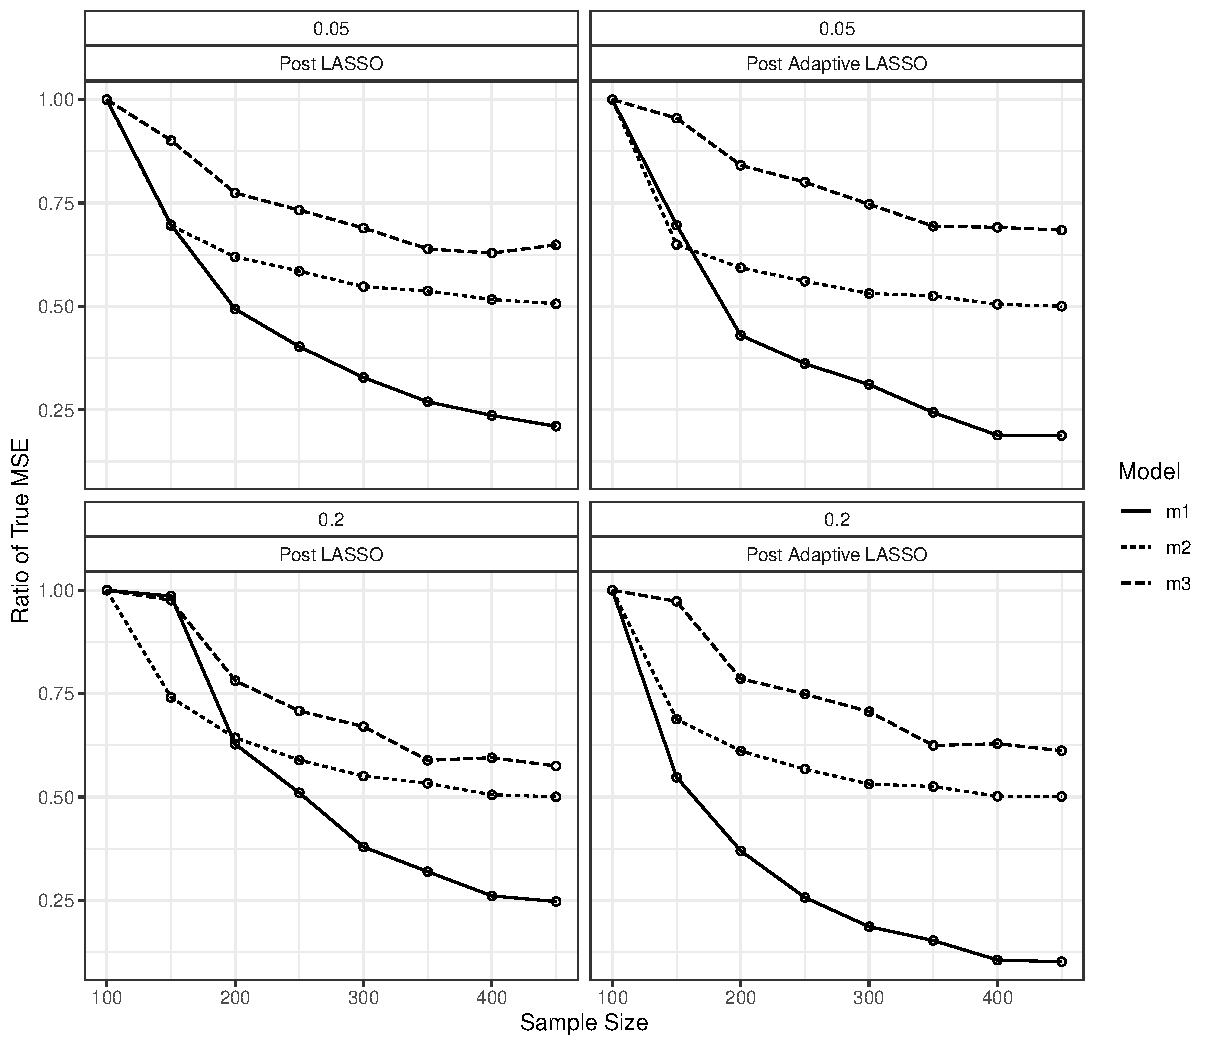
\includegraphics[width = 1.0\textwidth] {Graphics/rate.median.plot.pdf}
	%}
	\caption{Comparison of convergence rates (using median MSE)}
	\label{rate.median.plot}
    \end{figure}